\chapter{Hipótesis}

%La hipótesis que se maneja en este estudio se basa en la suposici\'on de que la materia oscura está compuesta de partículas elementales las cuales pueden ser producidas en los laboratorios modernos de física de part'iculas. De ser esto cierto se requiere de un nuevo marco teórico, es decir una extensión al modelo estándar que sustente dicha hipótesis. Afortunadamente ya se cuenta con modelos bien fundamentas que predicen dicha producción, uno de los modelos más populares es el conocido como "dark SUSY"~\cite{} en el cual existe un llamado sector oscuro donde por medio del rompimiento del grupo de simetría $U(1)_{D}$ se da lugar a la creación de fotones oscuros ($\gamma_{D}$) ligeros, los cuales interactuarían con partículas del modelo estándar y dicha fuerza de interaccion estaria descrita por medio de un parametro de mezcla cinetico $\epsilon$.  Una representacion grafica entre el sector oscuro y el del modelo estandar representa en la la Figura~\ref{fig:sketch_darksector} (izquierda). En "dark SUSY" ademas de particulas de materia oscura se da lugar a la producccion de particulas supersimetricas (SUSY), en donde la mas ligera de estas, el neutralino, dejaria de ser estable y podria decaer al foton oscuro. Las nuevas fuerzas en "dark SUSY" estarian mediadas mediante un termino de acoplamiento a la hypercarga del modelo estandar, descrito por la siguiente ecuacion.  

Si se hace supuesto que la materia oscura está compuesta de partículas elementales las cuales pueden ser producidas en los laboratorios modernos de física de partículas. De ser esto cierto se requiere de un nuevo marco teórico, una extensión al modelo estándar que sustente dicha hipótesis y el modelo conocido como "dark SUSY"~\cite{susy} en el cual predice un llamado sector oscuro donde por medio del rompimiento del grupo de simetría $U(1)_{D}$ se da lugar a la creación de fotones oscuros ($\gamma_{D}$) ligeros, los cuales interactuarían con partículas del modelo estándar y dicha fuerza de interacción estaría descrita por medio de un parámetro de mezcla cinético $\epsilon$.  Una representación gráfica entre el sector oscuro y el del modelo estándar representa en la la Figura~\ref{fig:sketch_darksector} (izquierda). En "dark SUSY" además de partículas de materia oscura se da lugar a la producción de partículas supersimétricas (SUSY), en donde la mas ligera de estas, el neutralino, dejarían de ser estable y podría decaer al fotón oscuro. 

Las nuevas fuerzas en "dark SUSY" estarían mediadas mediante un término de acoplamiento a la hipercarga del modelo estándar, descrito por la lagrangiana \cite{bb38,bb39}.

\begin{equation} 
L_{KM} = \frac{\epsilon}{2} F_{\mu\nu}^{\gamma}F^{D_{\mu\nu}}
\end{equation}

\begin{figure}
    \centering
    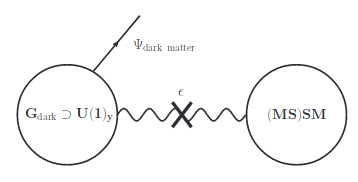
\includegraphics[width=0.4\textwidth]{HIPOTESIS/sketch_darksector.png}
    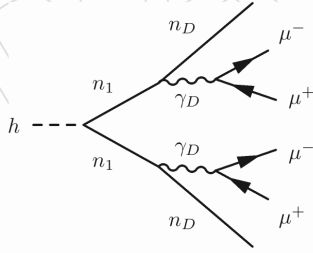
\includegraphics[width=0.4\textwidth]{HIPOTESIS/darksusy_feynman.png}
    \caption{. Ilustración esquemática de la conexión entre el sector oscuro y el modelo estándar, los cuales están conectados mediante un término de mezcla dinámica.}
    \label{fig:sketch_darksector}
\end{figure}

Donde $F_{\mu\nu}^{D}$ representa el campo oscuro y $\epsilon$ es un parámetro constante relacionado con la interacción.  De esta manera se obtiene como el fotón oscuro puede decaer a leptones \cite{bb41} del modelo estándar con una amplitud de decaimiento dada por:

\begin{equation}
  \Gamma_{\gamma D \rightarrow ll} = \frac{1}{3}\alpha \epsilon^{2} m_{\gamma D} \sqrt{1-\frac{4 m_{l}^{2}}{m_{\gamma D}^2}}(1+\frac{2m_{l}^{2}}{m_{\gamma D}}^{2})
\end{equation}

La expresión para las amplitudes permite calcular el tiempo de vida del fotos oscuro dado por: 

\begin{equation}
  \tau_{\gamma D}= \frac{\hbar}{\Gamma_{\gamma D Total}}=\frac{1}{\Gamma_{\gamma D \rightarrow e^{+}e^{-}}  + \Gamma_{\gamma D \rightarrow \mu^{+}\mu^{-}} + \Gamma_{\gamma D \rightarrow hadrons}}
\end{equation}

%%% EScribir la ecuacion. 




El diagrama de Feynman para el proceso del modelo "dark SUSY" $h\rightarrow 2n_{1}\rightarrow 2n_{D}\rightarrow 2\gamma_{D} \rightarrow 2n_{D} + 4\mu$ se muestra en la figura~\ref{fig:sketch_darksector} (derecha), el estudio de este proceso y la obtención de sus características (ver Figura \ref{fig:foton_oscuro}) permitiría inicializar escenarios extendidos de "dark SUSY" para estudios con versiones mas complejas que involucrarían otras partículas del sector oscuro como Higgs oscuros, o bosones Z y W oscuros, dando cabida a procesos como $pp\rightarrow h \rightarrow Z_{D}Z/Z_{D}Z_{D}/Z_{a}\rightarrow 4\mu$. %Sin embargo dichos modelos escapan a los alcances de esta tesis y podrian ser explorados en un analsis futuro. 

%Este escenario simple "dark SUSY" podria ser extendido de diversas maneras para estudios posteriores, como por ejemplo, en versiones mas complejas que involucrarían otras partículas del sector oscuro como Higgs oscuros, o bosones Z y W oscuros, dando cabida a procesos como $pp\rightarrow h \rightarrow Z_{D}Z/Z_{D}Z_{D}/Z_{a}\rightarrow 4\mu$. %Sin embargo dichos modelos escapan a los alcances de esta tesis y podrian ser explorados en un analsis futuro. 

\begin{figure}[h]
    \centering
   % 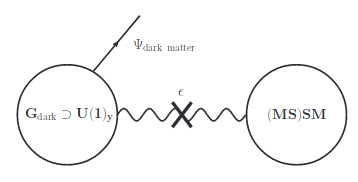
\includegraphics[width=0.4\textwidth]{HIPOTESIS/sketch_darksector.png}
    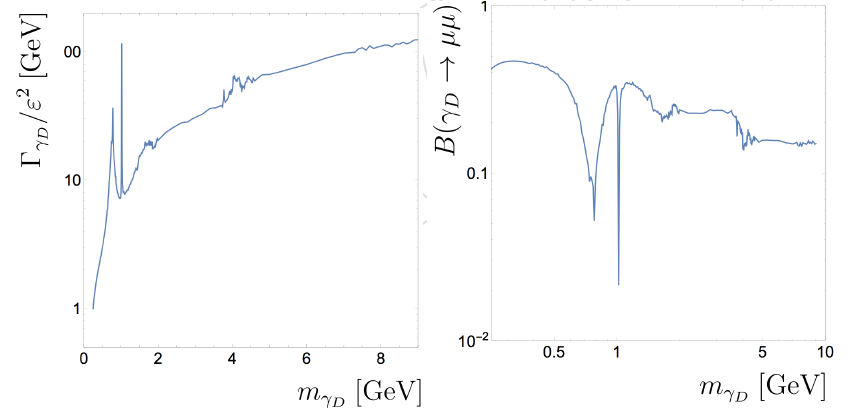
\includegraphics[width=0.8\textwidth]{HIPOTESIS/foton_oscuro.png}
    \caption{Izquierda: Peso total de los diferentes modos de desintegración del fotón oscuro, normalizado por $\epsilon^2$. Derecha: Probabilidad de decaimiento para $\gamma_D = \mu \mu$.}
    \label{fig:foton_oscuro}
\end{figure}














